\documentclass[letterpaper, 12pt]{article}
\usepackage{graphicx} % Required for inserting images
\usepackage{textcomp}
\usepackage{fullpage}
\usepackage{amsmath}
\usepackage{xcolor}
\usepackage{float}
\usepackage{geometry}
\usepackage{biblatex}
\geometry{margin=1in}
\usepackage{enumitem}
\usepackage{microtype}
\usepackage{gensymb}
\usepackage{parskip}
\usepackage{tikz}
\usepackage{caption}
\usepackage{cancel}
\usepackage{nicefrac}


\usepackage{hyperref}
\hypersetup{
  colorlinks=true,        % Enable colored links
  linkcolor=teal,         % Set color for internal links
  citecolor=teal,         % Set color for citations
  filecolor=teal,         % Set color for file links
  urlcolor=teal           % Set color for URLs
}

\usepackage[version=4]{mhchem}

\title{Protein structure and folding}
\author{BIOS 1006}
\date{20 June 2025}

\begin{document}

\maketitle

\section*{Objectives}

\begin{itemize}
\item Know all definitions.
\item Describe the types of reactions involving amino acids.
\begin{itemize}
\item Ionic reactions: negative + positive (acidic + basic)
\item Hydrogen bonding: polar + polar (hydrophilic)
\item Disulfide bonds: cysteine + cysteine
\item Peptide bonds: amino acid + amino acid, partial double bond character, rigid (not rotatable)
\end{itemize}
\item Describe properties of the bonds in the polypeptide backbone.
\begin{itemize}
\item Dihedral angles: $\phi$ (phi) angle/bond (N-C$_\alpha$), $\psi$ (psi) angle/bond (C$_\alpha$-C), and $\omega$ (omega) angle/bond (C-N)
\item Dihedral angles are rotatable, except for the peptide bond ($\omega$)
\end{itemize}
\item Describe and identify the different classes of protein structure: primary, secondary, tertiary and quaternary.
\begin{itemize}
\item Primary structure: unique sequence of amino acids in a polypeptide
\item Secondary structure: local folding patterns (e.g., $\alpha$-helices, $\beta$-strands)
\item Tertiary structure: overall 3D arrangement of all residues in a polypeptide
\item Quaternary structure: arrangement of multiple polypeptide subunits in a protein complex
\end{itemize}
\item Describe the importance of primary structure in protein folding and the relationships between proteins.
\item Describe the properties of features, such as secondary structure elements and motifs, that are found in proteins.
\item Describe the forces that stabilize tertiary and quaternary structures of proteins.
\item Describe the properties of different protein types, classifications and architectures.
\item Understand the role of free energy, dynamics, the forces involved and the factors that influence, aid or impede protein folding, shape and function.
\end{itemize}

\newpage

\section*{Protein structure}

\subsection*{Peptide/amide bonds}

\textbf{Dehydration synthesis} or \textbf{condensation reaction} or \textbf{nucleophilic substitution}

Nitrogen with a lone pair attacks the carbonyl carbon of another amino acid, forming a covalent bond and releasing water. This requires energy and a \textbf{ribozyme} (enzyme made out of nucleotides, RNA) called a \textbf{ribosome} to catalyze the reaction.

\subsection*{Resonance structures}

Electrons (usually in double or triple bonds, or lone pairs) can move around
and be ``shared'' or ``delocalized'' over two or more atoms. This is called \textbf{resonance}.

\textbf{Resonance hybrids} result in the...

\begin{itemize}
\item \ce{C-N} bond having \textbf{partial double bond character}.
\item peptide bond being shorter and essentially planar. (\ce{sp^2} hybridized, trigonal planar)
\end{itemize}

Resonance structures have characteristics of both arrangements.

\subsubsection*{Resonance structures of the peptide bond}

C$\alpha$ on opposite sides of the amide bond = \textbf{trans} conformation (preferred form in proteins)

C$\alpha$ on the same side of the amide bond = \textbf{cis} conformation (less common, leads to steric clashes)

\subsection*{Dihedral angles}

\begin{itemize}
\item \textbf{$\phi$ (phi) angle/bond}: nitrogen - $\alpha$ carbon, \ce{C-N-C_$\alpha$-C}
\item \textbf{$\psi$ (psi) angle/bond}: $\alpha$ carbon - carbonyl carbon \ce{N-C_$\alpha$-C-N}
\item \textbf{$\omega$ (omega) angle/bond}: carbonyl carbon - nitrogen \ce{C_$\alpha$-C-N-C_$\alpha$}
\item Rotatable
\end{itemize}

\textbf{The only bond that is not rotatable is the peptide bond (amide bond)} because it has partial double bond character due to resonance. This means that the \ce{C-N} bond is rigid and planar, which restricts the rotation of the peptide bond.

\subsection*{Key terms for peptides}

\begin{description}
\item [residue] an amino acid within a peptide
\item [peptide] molecule containing amino acids linked together
\item [oligopeptide] molecule containing less than 10 amino acids
\item [polypeptide] molecule containing more than 10 amino acids
\item [proteins] functional molecules consisting of one or more polypeptides
\end{description}

\subsection*{Levels of protein structure}

\subsubsection*{Primary structure}
The unique sequence of amino acids that defines a peptide or polypeptide; shows all covalent bonds.

\subsubsection*{Secondary structure}
$\alpha$-helices (cylinders/arrows) and $\beta$-strands (arrows, N- to C-terminus) are connected by random coils

\paragraph{The $\alpha$ helix} Looks like a spiral staircase, stabilized by hydrogen bonds between amide groups in the protein backbone. The hydrogen bonding pattern unique to alpha helix is that it requires hydrogen bonds between $i$ and $i+4$ (where $i$ is the amino acid of interest) and are stronger than the hydrogen bond between a regular amine and carboxyl group.

\begin{itemize}
\item 3.6 residues per turn
\item Pitch (distance between 2 identical points on adjacent turns): 5.4 Å (0.1 nm)
\item Rise (distance between 2 identical points on adjacent residues, pitch/residues per turn): 1.5 Å (0.15 nm)
\item Torsion angles: $\phi$ = $\sim$-60$\degree$, $\psi$ = $\sim$-45$\degree$
\item H-bonds parallel to helical axis and point in the same direction. The $\alpha$ helix has a dipole
\item R-groups point outwards
\item On average, $\sim$10 residues per helix
\item Directionality: left-handed and right-handed helices. $\alpha$ helix is a right-handed helix
\item ``Helical wheel'' representation of an $\alpha$-helix (a view down the helical axis)
\end{itemize}

\paragraph{The $\beta$ strand} \textbf{Different from $\beta$-sheets.} Link together to form $\beta$-sheets. Strands can have parallel (pointing in the same direction) or antiparallel (pointing in opposite directions) orientations. $\beta$ strands are stabilized by hydrogen bonds. The hydrogen bonding pattern unique to beta strands is that it requires hydrogen bonds between $i$ and $i+2$ (where $i$ is the amino acid of interest) and are weaker than the hydrogen bond between a regular amine and carboxyl group.

\begin{itemize}
\item Amino acids that interact can be distant in primary structure
\item Parallel: N $\to$ C and N $\to$ C, less ordered hydrogen bonds, angled, not collinear (weaker)
\item Anti-parallel: N $\to$ C and C $\to$ N, very ordered hydrogen bonds, perpendicular, collinear (stronger)
\item $\beta$-strands form $\beta$-pleated sheets
\item R groups on opposite sides of sheet
\item Amphipathic pattern: 1 polar (hydrophilic) - 1 nonpolar (hydrophobic)
\item $\psi$ = $\sim$-120$\degree$, $\phi$ = $\sim$120$\degree$
\end{itemize}

\paragraph{Less common secondary structures} The $\beta$-turn and left-handed helix are less common. The $\beta$ turn is a 4 amino acid motif with beta sheet-like characteristics, and left-handed helices are present in collagen.

\subsubsection*{Secondary structures on Ramachandran plot}

\begin{itemize}
\item Plots $\phi$ and $\psi$ values
\item 4 quadrants
\item Top left: $\beta$ sheets
\item Top right: left-handed $\alpha$-helix
\item Bottom left: right-handed $\alpha$-helix
\item Bottom right: disfavored
\end{itemize}

\begin{figure}[H]
\centering
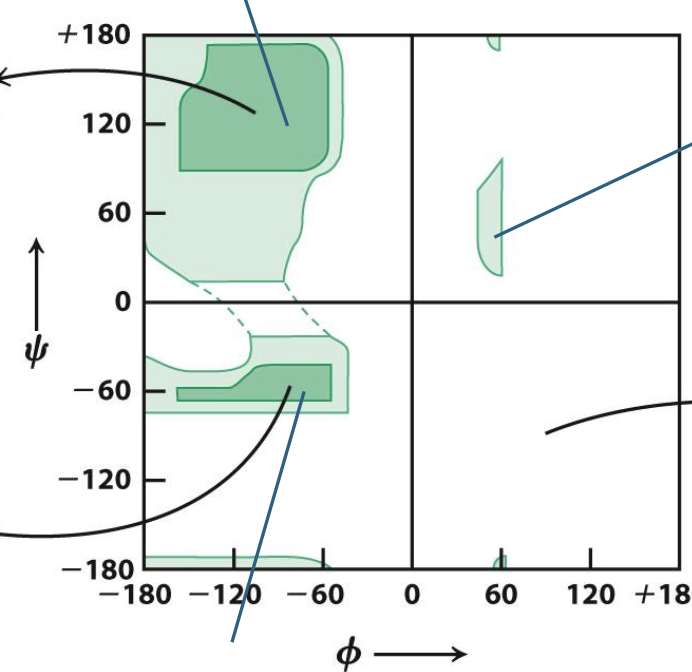
\includegraphics[width=0.7\textwidth]{ramachandran}
\end{figure}

\subsubsection*{Random coil region}
A flexible amino acid sequence that does not adopt a uniform secondary structure fold and can play essential roles in the structure and function of the protein.

\subsubsection*{Tertiary structures}
The three-dimensional arrangement of \textit{all} residues that comprise a polypeptide. 

\begin{itemize}
\item Results from \textbf{protein folding}, a process driven by primary structure, hydrophobic effect, and R group interactions
\item Tertiary structure is predominantly stabilized by electrostatic interactions (H bonds, salt bridges, van der Waals) and covalent bonds (disulfides)
\end{itemize}

\subsubsection*{Folded proteins}
\begin{itemize}
\item All-helical
\item All $\beta$ sheet
\item Mixed $\alpha$ and $\beta$
\end{itemize}

\subsubsection*{Anfinsen's hypothesis}
\underline{Primary structure drives protein folding}

\begin{itemize}
\item Added 8M urea to destroy hydrogen bonding in proteins and mercaptoethanol (reducing agent) to destroy disulfide bonds
\item Protein denatured
\item Hydrogen bonds and disulfide bonds began to re-form
\item Protein refolded
\end{itemize}

\subsubsection*{Hydrophobic effect drives protein folding}

\textbf{Hydropathy plot:}

\begin{figure}[H]
\centering
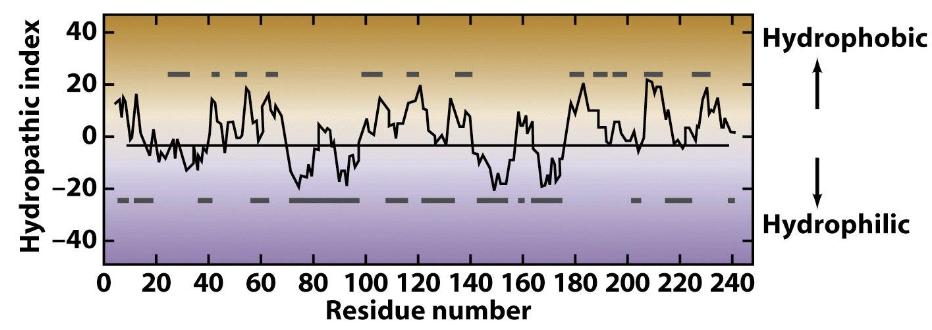
\includegraphics[width=0.7\textwidth]{hydropathy}
\end{figure}

Hydrophobic, higher values = in the core of the protein, embedded in the membrane

Hydrophilic, lower values = surface exposed

\subsubsection*{Quaternary structure}

The three-dimensional arrangement of polypeptide subunits in a protein complex containing two or more polypeptides

\textbf{Nomenclature:}

If all subunits are identical, \textbf{homo-} \\
If subunits are not identical, \textbf{hetero-} \\

2 subunits = dimer \\
3 subunits = trimer \\
4 subunits = tetramer \\
5 subunits = pentamer \\
6 subunits = hexamer

(Example: homodimer, heterotetramer, etc.)

\textbf{Oligomers} = 2 or more subunits are identical

\textbf{homo-oligomer} = all subunits are the same \\
\textbf{hetero-oligomer} = two or more different subunits \\
\textbf{protomer} = repeating structural unit

Association of subunits are often driven by hydrophobic effect. Quaternary structure is also stabilized by covalent bonds, salt bridges, hydrogen bonds, and van der Waals interactions.

\subsection*{Shape and stability}

\begin{itemize}
\item Non-polar amino acids side chains are forced into the interior of the protein by the hydrophobic effect
\item Van der Waals interactions organize and stabilize the core structure
\item Hydrophilic on the outside, hydrophobic on the inside
\item Ionic interactions form between proteins with different charges
\item Hydrogen bonds between R groups, R group -- water, and R group -- backbone
\end{itemize}

\subsubsection*{Globular proteins}

\begin{itemize}
\item Spherical or elliptical
\item Play enzymatic or regulatory roles
\item Water-soluble
\end{itemize}

\subsubsection*{Fibrous proteins}

\begin{itemize}
\item Rod-shaped
\item Play structural and protective roles
\item Water-insoluble (so your hair doesn't dissolve...)
\end{itemize}

\subsubsection*{Simple proteins}
Only composed of amino acids

\subsubsection*{Conjugated proteins}
Proteins that have a bound \textbf{prosthetic group} (not peptide-based) that is required for function. Covalently attached or IMF interaction

\textbf{apo-protein} prosthetic group is not present \\
\textbf{holo-protein} prosthetic group is present

\subsubsection*{Thermodynamics of protein folding}

\begin{itemize}
\item Driven by hydrophobic effect and primary structure (R group interactions)
\item Allows for proteins to be dynamic
\item Folded proteins are in equilibrium with less folded states
\item Lowest energy states are most populated
\item Dynamics are essential for proper folding and functioning
\item Proteins are not rocks!
\item Dynamic motions can do work
\end{itemize}

\subsubsection*{Intrinsically unstructured proteins}

\begin{itemize}
\item Few hydrophobic amino acids
\item High percentage of hydrophilic amino acids (glycine, proline)
\item May become structured upon post-translational modification or binding other biomolecules
\end{itemize}

\subsection*{Factors that influence protein folding}

\begin{itemize}
\item Primary structure!
\item Amino acid modifications
\item Temperature
\item pH
\item Size
\item Binding partners and prosthetic groups
\item Presence of \textbf{chaperones} (protein complexes that help in the folding of new proteins and old denatured proteins)
\end{itemize}

\subsection*{Denaturants}

\begin{itemize}
\item Acid or base - pH should be within 1 pH unit of the isoelectric point
\item Organic solvents (ethanol) - disrupt H-bonds in 2$\degree$
\item Detergents - disrupt protein core in 3$\degree$ and 4$\degree$
\item Reducing agents - break disulfide bonds
\item Heavy metal ions - disrupt salt bridges and bind cysteine
\item Temperature - disrupts all bonds, increases kinetic energy and hurts all IMFs
\item Salt concentration - a little helps increase protein stability, but increases hydrophobic effect too much, neutralizes charges on surface
\item Mechanical stress - disturbs intramolecular forces
\end{itemize}

\end{document}